
\section{Flow over a smooth downward step}

This is a standard textbook energy conservation type problem. Water flows over a flat bedded channel, then through a smooth downward step, and continues over a flat bottomed channel with lower bed elevation.

The bed is represented with a one dimensional domain over $[0,25]$ m, with topography
\begin{equation}
z(x)= \left\{ \begin{array}{ll}
 0.2 & ~\textrm{if}\quad x \leq 9 ,,\\
 0.2-0.1(x-9) & ~\textrm{if}\quad 9 \leq x \leq 11\,,\\
 0 & ~\textrm{otherwise}\,,\\
\end{array} \right.
\end{equation}
The stage is imposed at the downstream boundary, and the discharge is imposed at the upstream boundary.

The analytical height is found by solving the Bernoulli equation. The simplified Bernoulli equation is the following cubic equation
\begin{equation}
h^3 + \left(z - \frac{q^2}{2 g H^2} - H \right) h^2 + \frac{q^2}{2 g} = 0\,,
\end{equation}
where $H$ is the upstream height and $q=uh$ is the discharge or $x$-momentum. When the height $h$ has been found, the velocity is computed as $u=q/h$\,.

\subsection{Results}
For our test we impose a discharge-per-unit-width of 1m$^2$/s, and a downstream stage boundary condition of 1.0m. 

Representatives of the simulation results are given in the following three figures. The boundary regions are excluded from the plot because the inflow boundary takes some time to adapt to the analytical solution (which is to be expected as we don't enforce the depth or velocity directly there). There should be excellent agreement between the numerical and analytical solutions. 

\begin{figure}
\begin{center}
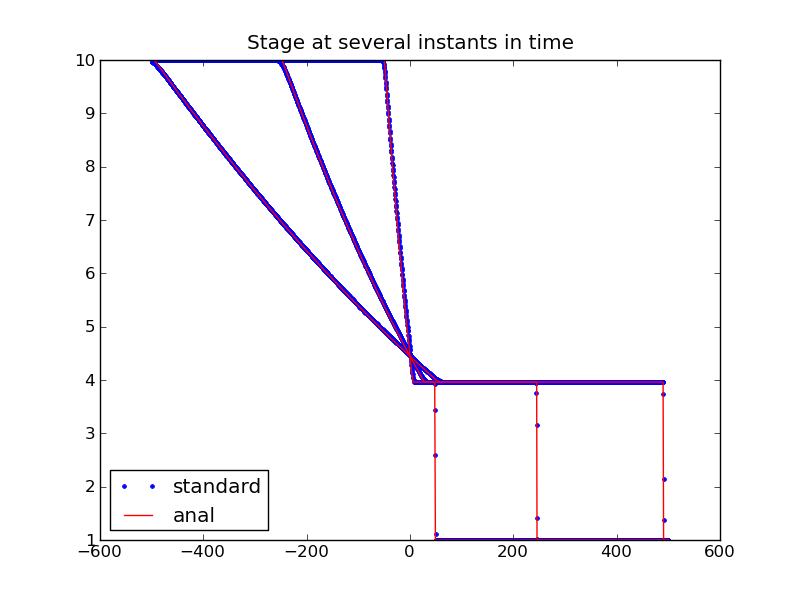
\includegraphics[width=0.9\textwidth]{stage_plot.png}
\end{center}
\caption{Stage results}
\end{figure}


\begin{figure}
\begin{center}
\includegraphics[width=0.9\textwidth]{xmom_plot.png}
\end{center}
\caption{Xmomentum results}
\end{figure}


\begin{figure}
\begin{center}
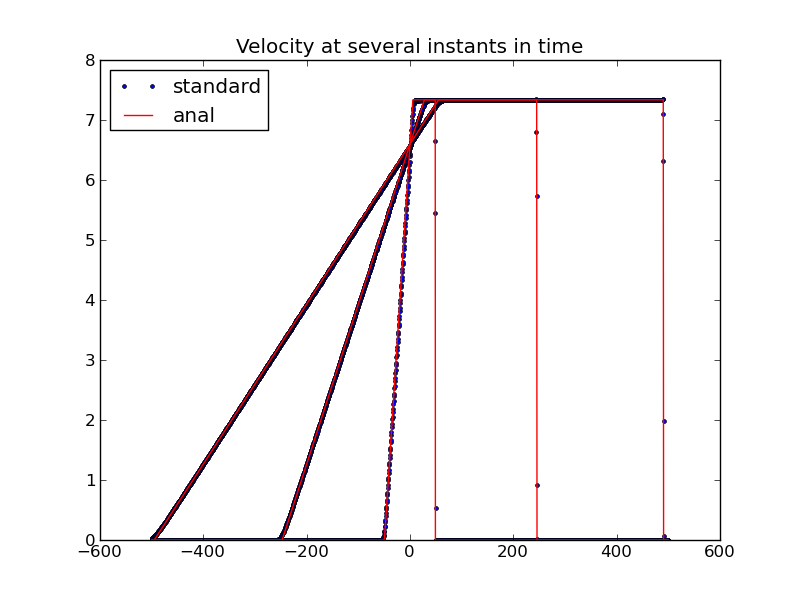
\includegraphics[width=0.9\textwidth]{xvel_plot.png}
\end{center}
\caption{Xvelocity results}
\end{figure}


\endinput
